\begin{frame}
	\begin{enumerate}
		\item korpusz: TED magyar-angol feliratok
	
		\item fordító csomag: NLTK translate package
		
		\item Dill szerializáló csomag
		
	\end{enumerate}
\end{frame}


\begin{frame}{Korpusz}
	TED korpusz:
	\begin{itemize}
		\item 360 ezer mondat pár
		\item XML formátum
		\item mondatok szintjén megfeleltetve egymásnak (aligne)
		\item szavak szintjén nincs megfeleltetés
	\end{itemize}
	
	\begin{figure}
		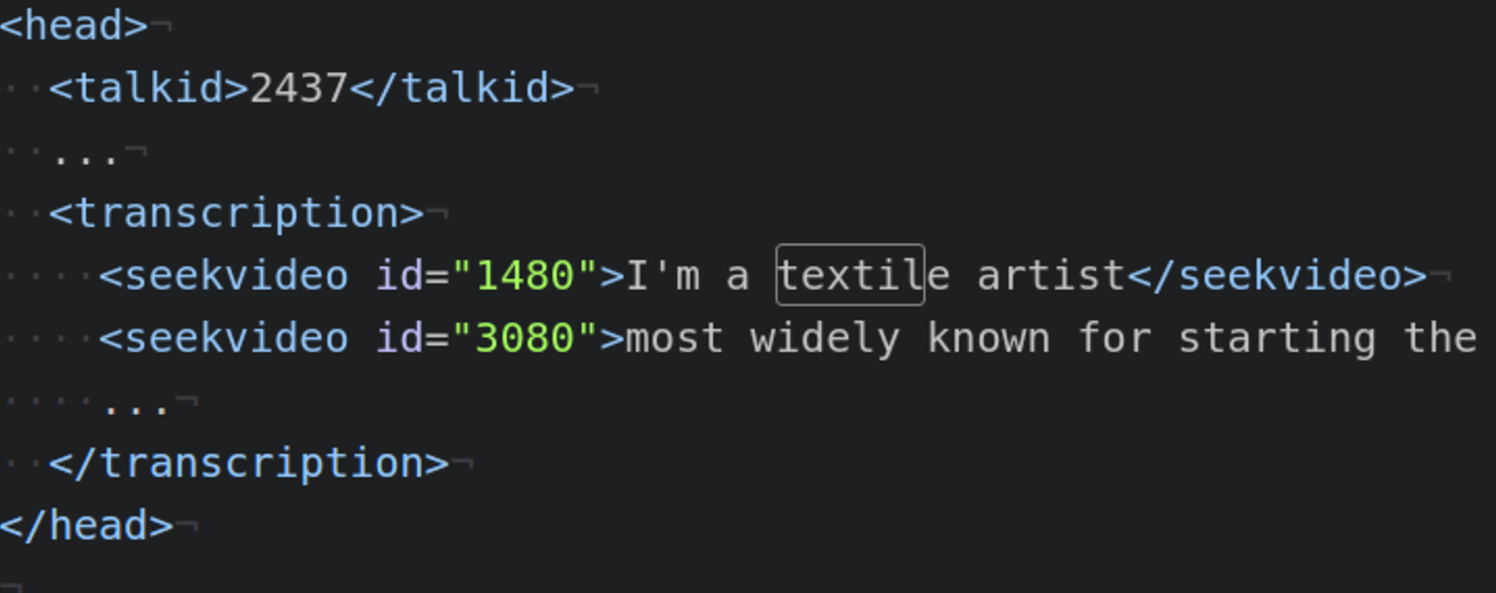
\includegraphics[width=1\textwidth,center]{images/ted}		
	\end{figure}
\end{frame}

\begin{frame}{NLTK translate package}

	\begin{enumerate}
		\item sentence pairs
		\item ibm2 model, bitext
		\item phrases, phrasetable
		\item language model
		\item StackDekoder
	\end{enumerate}

\end{frame}

\begin{frame}{Sentence pairs}
	\begin{itemize}
		\item XML parseolás
		\item mondatok előfeldolgozása -- írásjelek, felesleges fehér karakterek kiszűrése
		\item megfelelő mondat párok megfeleltetése egymásnak az id alapján
	\end{itemize}

\end{frame}

\begin{frame}{IBM2 model, bitext}
	IBM2:
	\begin{itemize}
		\item model felépítése a sentence paire-ekből
		\item bitext felépítése -- AlignedSent-ekből álló lista -- (words, mots, alignment)
	\end{itemize}
	
	Bitext:
	\begin{itemize}
		\item None-ok eltávolítása
	\end{itemize}
\end{frame}

\begin{frame}{Phrases, PhraseTable}
	Phrases:
	\begin{itemize}
		\item phrasek létrehozása a korpuszban található mondat párokból és ezek alignmentjéből
		\item kellenek a PhraseTable létrehozásához valamint a language model felépítéséhez
		\item ((0, 2), (0, 4), 'michael assumes', 'michael geht davon aus')	
	\end{itemize}
	
	PhraseTable:
	\begin{itemize}
		\item $f_i, e_i$ phrase párokat tartalmaz, valamint a hozzuk tartozó $translation$ $probabilityt$
		\item translation probability = $f_i$-ből $e_i$-be fordítható phrasek szám / $f_i$ phrasek száma
	\end{itemize}
	
\end{frame}

\begin{frame}{Language model}
	\begin{itemize}
		\item a fordított mondat folytonosságát biztosítja
		\item valószínűséget rendel a célnyelvbeli phrasekhez
		\item a valószínűségeket bi-grammok és a chain modell segítségével számolja
	\end{itemize}
	\begin{equation}
		P(w_2|w_1) = \frac{count(w_1, w_2)}{count(w_1)}
	\end{equation}
\end{frame}

\begin{frame}{StackDekoder}
	\begin{itemize}
		\item a PhraseTable-ből és language modellből hozható létre
		\item optimumkeresést végez a PhraseTable-en a language modell segítségével (EZ ITT NEM TELJESEN HELYES!!!!!)
		
	\end{itemize}
\end{frame}

\begin{frame}{Szerializáció}
	???????
\end{frame}